
\documentclass[12pt]{article}

\usepackage{graphicx}
\begin{document}
\title{Network Security Project Report}
\author{Shuo Li sli53@jhu.edu Yuge Gong ygong@jhu.edu}
\date{\today}
\maketitle
\section{DDos Attack}

\subsection{DDos Detection}

\begin{figure}
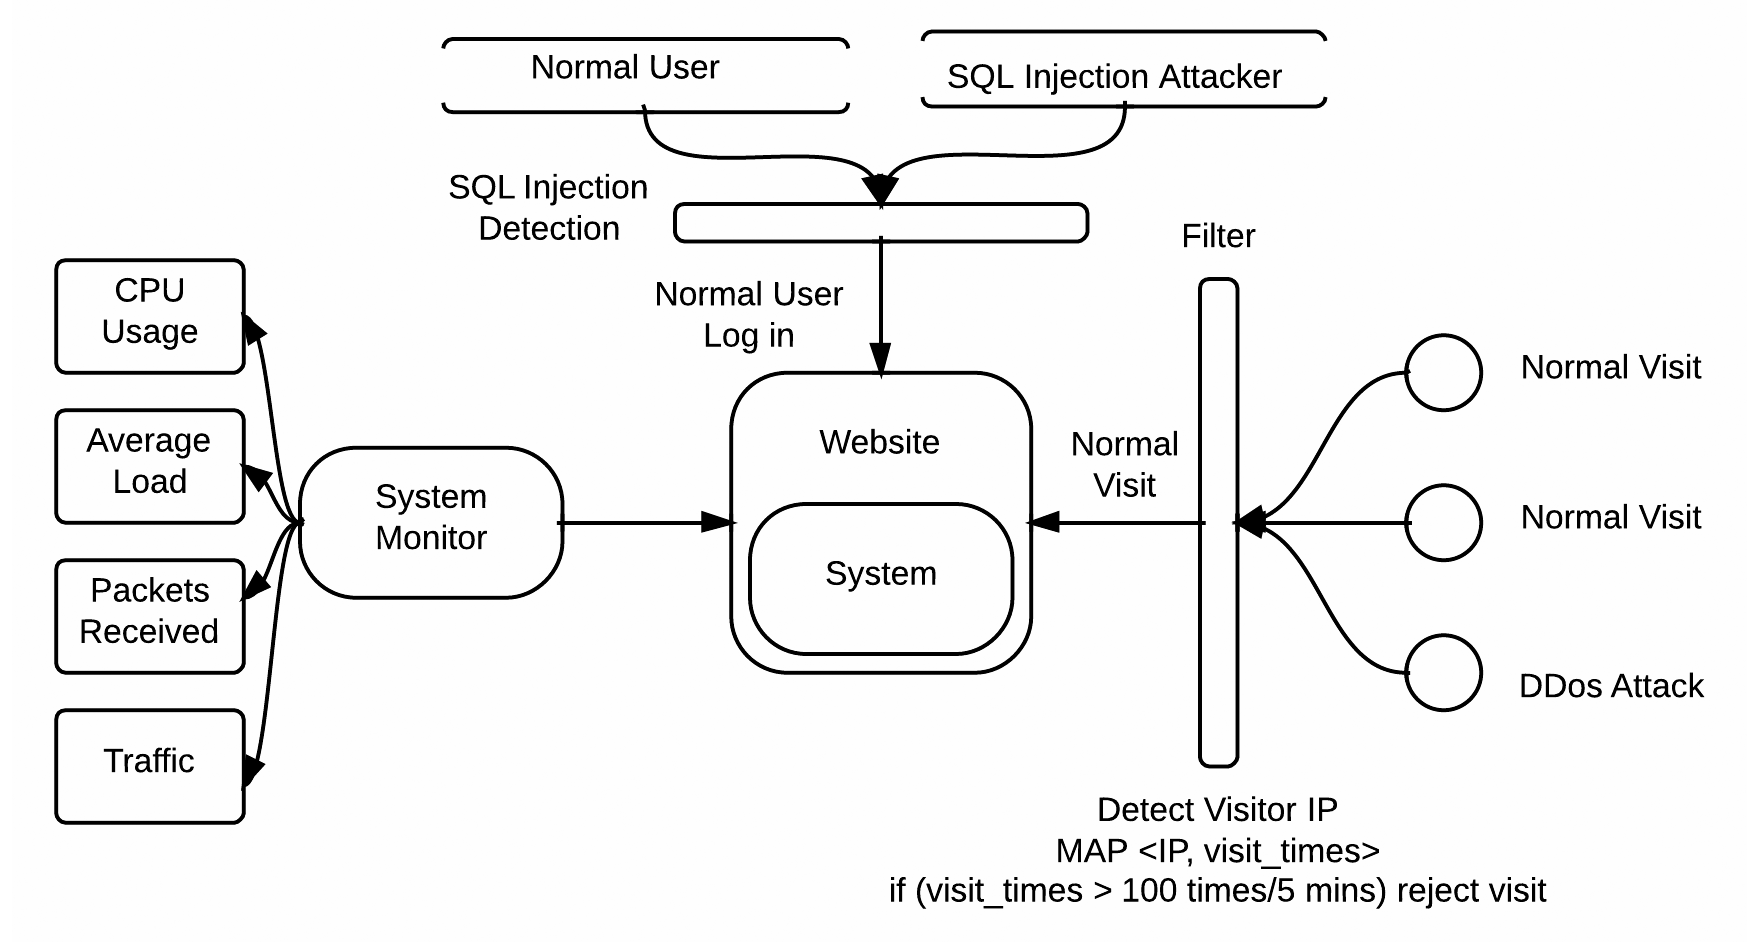
\includegraphics[scale=0.23]{flowchart.png}
\caption{System flow chart}
\end{figure}


\makeatletter\def\@captype{table}\makeatother
\begin{minipage}{.60\textwidth}
\centering
\caption{Website without DDos detection}
\begin{tabular}{|c|c|c|c|}
\hline
  CPU Usage & Avg Load & Packets & Traffic
 \\
  \hline
  3.12 & 0.62 & 194 & 0 \\
  3.33 & 0.66 & 270 & 0\\
  5.88 & 0.71 & 266 & 0\\
  6.45 & 0.67 & 286 & 5\\
  6.25 & 0.78 & 274 & 0\\
  8.82 & 0.77 & 267 & 0\\
  6.45 & 0.71 & 354 & 0\\
 30.00 & 0.90 & 358 & 0\\
  14.7 & 0.73 & 291 & 0\\
  6.45 & 0.85 & 306 & 0\\
  6.60 & 0.88 & 364 & 0\\
  9.90 & 0.84 & 270 & 0\\
  8.82 & 0.82 & 345 & 0\\
  9.37 & 0.98 & 494 & 0\\
  9.37 & 0.78 & 378 & 0\\
 75.00 & 1.07 & 637 & 1\\
 30.00 & 1.00 & 459 & 0\\
 30.95 & 1.00 & 359 & 0\\
 23.70 & 0.73 & 315 & 0\\
    \hline
\end{tabular}
\end{minipage}
\makeatletter\def\@captype{table}\makeatother
\begin{minipage}{.60\textwidth}
\centering
\caption{Website with DDos detection}
\begin{tabular}{|c|c|c|c|}
\hline
  CPU Usage & Avg Load & Packets & Traffic
 \\
  \hline
  3.12 & 0.69 & 163 & 0 \\
  3.12 & 0.71 & 280 & 0\\
  6.25 & 0.75 & 165 & 0\\
  3.22 & 0.80 & 7632 & 5\\
 10.25 & 0.74 & 315 & 0\\
  8.33 & 0.78 & 177 & 0\\
  6.60 & 0.87 & 8809 & 7\\
  9.90 & 0.81 & 8933 & 6\\
  8.33 & 0.90 & 8878 & 6\\
 13.15 & 0.91 & 16250 & 12\\
 12.50 & 0.99 & 16388 & 12\\
 11.76 & 0.99 & 16810 & 12\\
 10.25 & 0.91 & 17738 & 13\\
  9.37 & 1.00 & 17859 & 13\\
 10.81 & 1.99 & 16841 & 13\\
 70.31 & 1.00 & 13009 & 9\\
  9.90 & 0.99 & 10418 & 8\\
 13.51 & 1.15 & 11876 & 9\\
 10.81 & 1.14 & 9329 & 7\\
    \hline
\end{tabular}

\end{minipage}
\subsection{DDos Defense}


\newpage
\section{SQL Injection}

In SQL injection part, a website written by jsp was build to implement SQL injection. This website is a one with simple functions that normal users can log in this website by using their own user name and password. If the user name and password match with each other, then the web server will redirect the user to a new web page showing that "Log in successfully!", otherwise, the web server will feedback an error message.\\

Attackers, on the other side, are trying to log in this website by malicious input of user name or password. What we would do is finding out the method to detect attackers' attacks and defend them. In order to show the effects of the detection and defense of SQL injection for this website, we build two login pages for comparison. One is a naive website checking only the length of the input strings, which cannot be zero or larger than 15. The other is equiped with serveral methods of SQL injection detection and defense.\\

\subsection{SQL Injection Detection}

Before we detect SQL injection, we need to understand how a SQL Injection happens. Let's first have a look at how a website without detection works when someone input his user name and password to log in.\\

In this project, we have used MySQL to build a dabase for the website and keep a table named ``\verb"Tbl_User"'' for user informations including user name and matching password.\\

Suppose one user Tom wants to log in the website, he would fill the log in form with his user name ``Tom'' and the matching password ``Tom1234''. After he submits his information, the web server would then begin to parse these informations. Actually, in the jsp page of log in, there are following java sentences to explain this procedure. \\

\begin{enumerate}
\item \verb"String user = request.getParameter(``userid'');"
\item \verb"String pwd = request.getParameter(``pwd'');"
\item \verb"String query = ``SELECT * FROM Tbl_User WHERE u_id = `''"\\
      \verb"+ user +``' AND u_password = `'' + pwd +``';'';"
\item \verb"ResultSet rs = st.executeQuery(query);"
\end{enumerate} 

The first and second sentence are used to get the user name ``Tom'' and the password ``Tom1234'' input from user Tom. The third sentence combines the input strings with the incomplete SQL query. After we get the query, ``SELECT * FROM \verb"Tbl_User" WHERE \verb"u_id" = 'Tom' AND \verb"u_password" = 'Tom1234';''(setence 3), we would use it to do searching on database based on the informations provided in sentences above(sentence 4).\\

Normally, a good person would provide legal informations, that is, a username and a password that had already been stored in database before. Then the server would use these informations to do SQL query to verify whether these informations are matching those in the database. However, a website attacker can utilize this verifying procedure to log in the website without verification. We will explain it then.\\

The main idea of SQL injection is to modify the SQL query of web server want to deal with. As the website without detection will not check the user inputs, any input will be accepted by server as long as the length of the input satisfying the requirements. Take an malicioius input of username as a SQL injection example. An attacker cannot just input ``Alice'' as his user name because the database does not store such a user name or the attacker cannot provide a matching password for the existing user name ``Alice''. To continuing his attacking, he can input ``\(1'\) OR \('1'\) = \('1'\)' instead of ``Alice''. Then he can input any password (except an empty one) to log in the website without any forbid. This is because the server is now doing the SQL query `` SELECT * FROM \verb"Tbl_User" WHERE \verb"u_id" = \('1'\) OR \('1'\) = \('1'\) AND \verb"u_password" = \('anyword'\) ''. As \('1'\) = \('1'\) will be true under any condition, the attacker can always log in the website without verification.\\

After knowing how an attacker user SQL injection to attack the website, we can then develop the method to detect the situation. In our case, we use regular expression([\verb"^0-9a-zA-Z"]) to check user's input. Relevant java sentences are shown as follows.\\

\begin{enumerate}
\item \verb"String regEx = ``[^0-9a-zA-Z]'';"
\item \verb"Pattern pattern = Pattern.compile(regEx);"
\item \verb"Matcher userMatcher = pattern.matcher(user);"\\ 
      \verb"Matcher pwdMatcher = pattern.matcher(pwd);"
\item \verb"if (userMatcher.find() $||$ pwdMatcher.find())"\\
      \verb"out.print(``<script> alert(`illegal characters!');"\\
      \verb"window.location='Login.jsp';</script>'');"
\end{enumerate} 

If a user name or password contains any character that is not a letter or figure, then the server would determine that the input contains illegal character(s) and then redirect the user to the original login page. Thus, the username or password is invalid and cannot be used to log in the website.\\

\subsection{SQL Injection Defense}

Using regular expression can standardise the input from users, which means implementing a detection of SQL injection can filter the malicious input from attackers to a large extent. Detection, however, cannot promise server a prevention of a SQL injection. A more efficient and safer way to defense attacker from SQL injection is being used here.\\

Instead of using simple SQL query to do search on database, we prefer prepared statements and storage procedure here. By implementing prepared statements, we can first define our SQL query, which make attacker cannot modify our SQL query later. By implementing a storage procedure, server will not just patch the incompleted SQL query sentense with input strings from users to get a completed one. On the other hand, we will regard these input string as input parameters of a single storage procedure stored in database before. \\

\begin{enumerate}
\item \verb"String user = request.getParameter(``userid'');" 
\item \verb"String pwd = request.getParameter(``pwd'');"
\item \verb"CallableStatement cs = con.prepareCall(``{CALL verifyUser(?,?)}'');"
\item \verb"cs.setString(``user'', user); cs.setString(``pwd'', pwd);"
\item \verb"ResultSet rs = cs.executeQuery();"	
\end{enumerate}

In the first two sentenses, the web server can get the input strings of user name and password as before, but then we will not use the simple query like ``SELECT * ...'' sentence any more. Instead, we would first define our parameterized query(sentence 3), then we set parameters for this prepared statements(sentence 4). After this, we call the storage procedure ``verifyUser''(sentence 5). By doing so, we can avoid using the input strings from users directly, which can reduce the posibility of SQL injection on server.\\

The following tables shows the differences between website reaction with or without SQL injection detection and defense.

\begin{table}[htbp]
\centering
\caption{Website without SQL injection detection}
\begin{tabular}{ l l   p{9cm}  }
\hline
  Input Username & Input Password & Reaction \\
  \hline
   & & Username cannot be empty! \\
  Alice & &Password cannot be empty!Wrong password!  \\
  Yuge & admin & Log in successfully! \\
  1' OR '1' = '1 & Any Password & Wrong password! \\
  1' OR '1' = '1 & 1' OR '1' = '1 & Log in successfully! \\ 
    \hline
\end{tabular}
\end{table}

\begin{table}[htbp]
\centering
\caption{Website with SQL injection detection}
\begin{tabular}{ l l   p{9cm}  }
\hline
  Input Username & Input Password & Reaction \\
  \hline
   & & Username cannot be empty! \\
  Alice & &Password cannot be empty!Wrong password!  \\
  Yuge & admin & Log in successfully! \\
  1' OR '1' = '1 & Any Password & lllegal characters! \\
  1' OR '1' = '1 & 1' OR '1' = '1 & lllegal characters! \\ 
    \hline
\end{tabular}
\end{table}

\newpage
\section{Reference}

\end{document}

